
\section{Introduction}

This paper presents the results of a field study of the Software Engineering Method and Theory (SEMAT) Essence framework \cite{SEMATKernel, EssenceBook} investigating the Essence kernels' novel approach to monitoring and steering software development projects. One of the promises of the approach lies in its potential ability to monitor any type of project holistically based on universal project states and steer these projects based on universal goals, hence making the monitoring and steering mechanisms independent from the method (such as Scrum \cite{AgileProjectManagement} and XP \cite{ExtremeProgramming2000}) or set of practices adopted by the project team.

We are interested in understanding the strengths and weaknesses of Essence by gaining experience of using the approach on real projects. We conducted a field study involving seven co-located and distributed student teams working on industrial projects. These students finish their graduate program with a project course at Carnegie Mellon University in Silicon Valley in the context of the Master of Science in Software Engineering program. During the project each student has the opportunity to apply the software engineering skills acquired throughout the program to solve a real industry problem. Monitoring and steering projects with the Essence kernel allows the researchers to identify where value is added for an educational program. Student team projects serve as a possible metaphor for newly formed industry team projects; the value added for a student team could transfer to an industry team.

As faculty, we allow teams to be self-organizing and responsible for their decisions, yet at the same time expect them to incorporate generally accepted software engineering practices, and demonstrate the ability to effectively steer their project. Each team manages its own project with minimal faculty supervision. In the past, the faculty observed that with minimal supervision some teams revert to old habits \cite{BareissTransferable}. As soon as the starting bell sounds, they can act as racetrack horses running towards the finish line with blinders, ignoring what they have learned in class and without concerns for software engineering discipline. The new freedom and the chance to write code for a client lead them to focus mostly on implementation and therefore to adopting a suboptimal way of working.

Our research hypothesis contends that Essence's monitoring and steering approach provides a lightweight framework for students to look at their project holistically, helping them to address various project dimensions beyond implementation. We stipulate that the framework acts as a routine reminder about applicable software engineering practices covered in previous courses, and this without being prescriptive and while being method agnostic. For instance, by using this technique, we expect students to think about involving stakeholders, improving the team's way of working, and demonstrating that the software system has the desired quality characteristics.

This paper reviews SEMAT's Essence framework and kernel, describes the field study planning and execution, reports on the analysis and interpretation of the field study data, recommends effective practices for introduction of Essence to a software engineering curriculum, and summarizes the conclusions.

\section{SEMAT ESSENCE OVERVIEW}
In 2009, Ivar Jacobson, Bertrand Meyer, and Richard Soley started work on the \quotes{Software Engineering Method and Theory} (SEMAT) with the goal of \quotes{re-founding software engineering as a rigorous discipline} \cite{JacobsonCallForAction}. While many software engineering principles, techniques, practices and methods exist, the SEMAT founders' ambition is to create a general theory of software engineering and a unifying process framework. Out of their initiative has emerged the SEMAT Essence language and kernel, which became an Object Management Group (OMG) beta standard in 2013.

The core idea of Essence is that software projects exhibit universal behavior and transition through identifiable states as they progress. Essence groups these states together by different software engineering aspects or dimensions called \quotes{alphas.} Essence identifies seven alphas as core to every software engineering project: \textbf{Stakeholders}, \textbf{Opportunity}, \textbf{Requirements}, \textbf{Software System}, \textbf{Team}, \textbf{Way of Working}, and \textbf{Work}. These seven alphas serve as the Essence kernel as illustrated in Figure \ref{EssenceKernel}.

\begin{figure}[h]
\centering
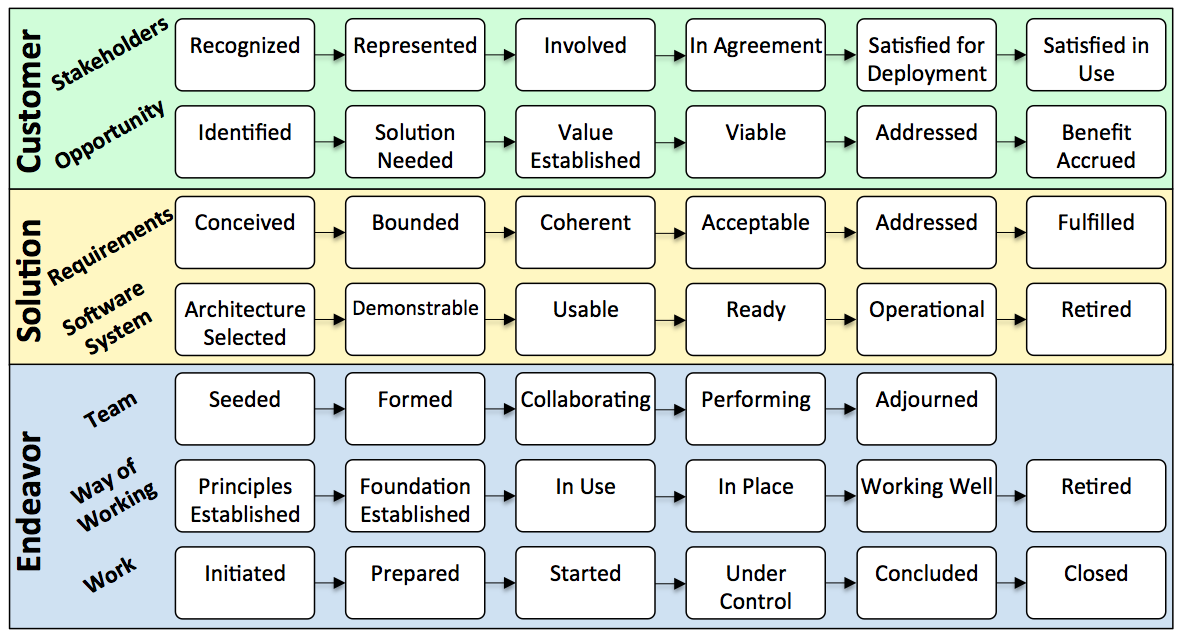
\includegraphics[width=3.30in]{project_steering_images/EssenceKernel.png}
\caption{Essence kernel alphas and their states }
\label{EssenceKernel}
\end{figure}

Each alpha progresses through a number of states during the project lifecycle. For example, the \textbf{Stakeholders} alpha progresses through the states \textit{Recognized}, \textit{Represented}, \textit{Involved}, \textit{In Agreement}, \textit{Satisfied for Deployment}, and \textit{Satisfied in Use}. Each state includes a checklist to help determine if the project has achieved that state. Each checklist item provides a goal to be reached in order to progress to that state.

Despite the sequential definition of the states for each alpha, in practice, projects could fall back to previous states. Similarly, in some circumstances, it might make sense for a project to achieve a number of states simultaneously within a given alpha.

The SEMAT vision is also to create a library of practices described using the Essence language and sitting on top of the Essence kernel. Practices would be composed to become specific methods addressing specific project or organization needs. Practices would help a team identify how to progress their project from one state to the next.

In The Essence of Software Engineering \cite{EssenceBook}, the authors identify three separate applications of Essence: 1) project monitoring and steering, 2) determining when to green light projects, and 3) describing workflow through an organizational structure. This paper focuses mostly on the first application, project monitoring and steering, where a team assesses its current project state in each of the alphas and identifies possible actions to help transition from the current state to the next target state.

\section{Field Study Description}
\label{Field Study Description}

The study focuses on understanding what value do project teams receive from following the SEMAT Essence's monitoring and steering approach provided by the kernel alphas and their states. Essence was introduced to master students at the beginning of their practicum projects. The students had no prior knowledge of Essence.

Using the goal template from GQM \cite{GQM}, our research goal is to:

\begin{table}[h]
\renewcommand{\arraystretch}{1.3}
\centering
\begin{tabular}{|p{1.20in}|p{1.90in}|}
\hline
\textbf{Analyze} & SEMAT Essence's monitoring and steering approach provided by the kernel alphas and their states \\ \hline
\textbf{for the purpose of} & evaluation \\ \hline
\textbf{with respect to its} & effectiveness \\ \hline
\textbf{from the point of view of the} & project team, educator, and researcher \\ \hline
\textbf{in the context of} & the software engineering practicum graduate course at Carnegie Mellon University. \\
\hline
\end{tabular}
\end{table}
 
This paper decomposes this goal into the following questions:

\textbf{Research Question 1}: Does the SEMAT Essence's monitoring and steering approach provide value to the project team?

\textbf{Research Question 2}: How does the approach provide value to the project team?

\textbf{Research Question 3}: When in the project lifecycle does the approach add value?

\textbf{Research Question 4}: What are the limitations to the approach's effectiveness?

The first section below describes the context of each project involved during the field study. The second section presents how Essence was introduced to the teams, either incrementally or using a workshop approach. The final section describes how the teams have been leveraging Essence during the remaining of their project.

\subsection{Practicum Projects' Context}


\begin{table*}[t]
\centering
\renewcommand{\arraystretch}{1.4}
\caption{Practicum projects' context}
\label{PracticumProjectsContext}
% \begin{tabular}{|p{0.6in}|p{1.1in}|p{1.1in}|}
\begin{tabular}{|p{0.75in}|p{1.05in}|p{0.3in}|p{1.05in}|p{0.7in}|p{2.3in}|}
\hline
\textbf{Team Name} &
\textbf{Industry Project} &
\textbf{Team Size} &
\textbf{Team Distribution} & 
\textbf{Average Work Experience} &
\textbf{Technical Complexity} \\
\hline
\hline
\multicolumn{6}{|l|}{\textbf{First Pilot Projects}} \\ 
\hline

Distributed-1 & 
Rendering of audio streams for accessibility purpose &
3 &
Distributed within same time zone &
10 years &
Integration with legacy code on a single platform involving C, HTML5 and open-source technology. \\
\hline

Distributed-2 & 
Access and preservation of electronic journals & 
4 & 
Distributed across 2 time zones & 
6 years &
Integration with legacy code on a single platform involving Java, MongoDB, Apache Jena and open-source technology. \\
 \hline

Distributed-3 & 
Survivable social network & 
4 & 
Distributed across 2 time zones & 
8 years &
Multi-platform involving Ruby on Rails, Javascript, jQuery Mobile. Embedded system constraints. \\
\hline

\multicolumn{6}{|l|}{\textbf{Second Pilot Projects}} \\ 
\hline

Co-located-1 & 
Electric vehicle fleet management & 
2 & 
Co-located & 
3 years & 
Green-field development involving Query, Node.js and MongoDB. Integration with Rest APIs for two vehicle brands. \\
\hline

Co-located-2 & 
Sonification of financial trading information & 
4 & 
Co-located & 
3 years & 
Integrates with third party APIs (Yahoo! and Google Finance). Involves Objective C, Ruby on Rails, iOS, Google App Engine and Python. Requires financial knowledge. Has a special focus on user experience. \\
\hline

Co-located-3 & 
Mobile performance testing & 
3 & 
Co-located & 
4 years & 
Xcode, Instruments, Eclipse, iOS 6.0, Android 4.2, jQuery Mobile, HTML5, Benchmark.js, Appception, Pivotal tracker, Redmine, GitHub, RubyMine, Rails 3.2, Ruby 1.9.2. Heroku, Amazon EC2, HighCharts.js, CSS3, Cordova \\
\hline

Co-located-4 & 
Virtual sensors definition and management & 
5 & 
Co-located & 
5 years & 
Multi-platforms involving HTML5, Javascript and j2ee. \\
\hline

\end{tabular}
\end{table*}


The authors introduced Essence to seven student teams: three geographically distributed student teams, referred as Distributed-1 to Distributed-3 for the purpose of this paper, and four co-located student teams, referred as Co-located-1 to Co-located-4. As shown in Table \ref{PracticumProjectsContext}, each team worked on creating or evolving a software solution for a different client, like an electric car fleet management system or a survivable social network. By design, the projects had a medium to high level of technical complexity, as they often involved multiple technologies or platforms or integrate with legacy systems.

The geographically distributed, part time students were working professionals with an average of eight years of development experience. Their practicum projects ran for 15 weeks, during which each student dedicated about 20 hours per week to the project. They worked in small teams of three to four members distributed across one or two time zones.

The co-located, full time students were at the beginning of their career with an average of four years of development experience. Their practicum projects ran for 12 weeks, during which each student dedicated about 20 hours per week to the project. They worked in co-located teams of two to five members.

The course syllabus imposed a few milestones and deliverables (like roadmap, statement of work, reflection report, and working software), with potential additional requests coming from the client. Teams determined their own software development approach. Most students had a reasonable knowledge of a diverse set of generally accepted software engineering practices, and the ability to execute these practices somehow effectively. All projects adopted an iterative lifecycle.

Even though the student population was quite diverse in terms of origin and culture, by the time the students started their practicum project they were immersed in the North American culture for at least eight months.

Table \ref{PracticumProjectsContext} summarizes the context of each practicum project in terms of the following dimensions \cite{AmblerDAD, BoehmBalancingAgilityAndDiscipline, KruchtenContextualizingAgile}: team size, team distribution, average work experience, and technical complexity.

Essence was introduced to the geographically distributed teams in the context of a first set of pilot projects, and to the co-located teams in the context of a second set of pilot projects

\subsection{Introducing Essence on Practicum Projects}
\subsubsection{First Pilot Projects - Incremental Approach}
In the Spring 2013 semester, the authors introduced the SEMAT Essence framework to three geographically distributed student teams at the beginning of the project. Because first impressions are critical for adoption, and because the researchers were uncertain of the value provided by Essence, we made the decision of introducing the framework with minimum overhead to avoid adoption resistance and minimize potential waste.

We briefly introduced Essence to all students using a slide presentation of about 20 minutes. Since the teams were distributed, a set of physical Essence cards was sent to each student, and a digital Essence board was created using Google Drawing (see Figure \ref{DigitalEssenceBoard}). The digital board included one row for each of the seven alphas in the Kernel. Each row contained the sequence of states that the alpha progresses through during the project lifecycle.

\begin{figure}[t]
\centering
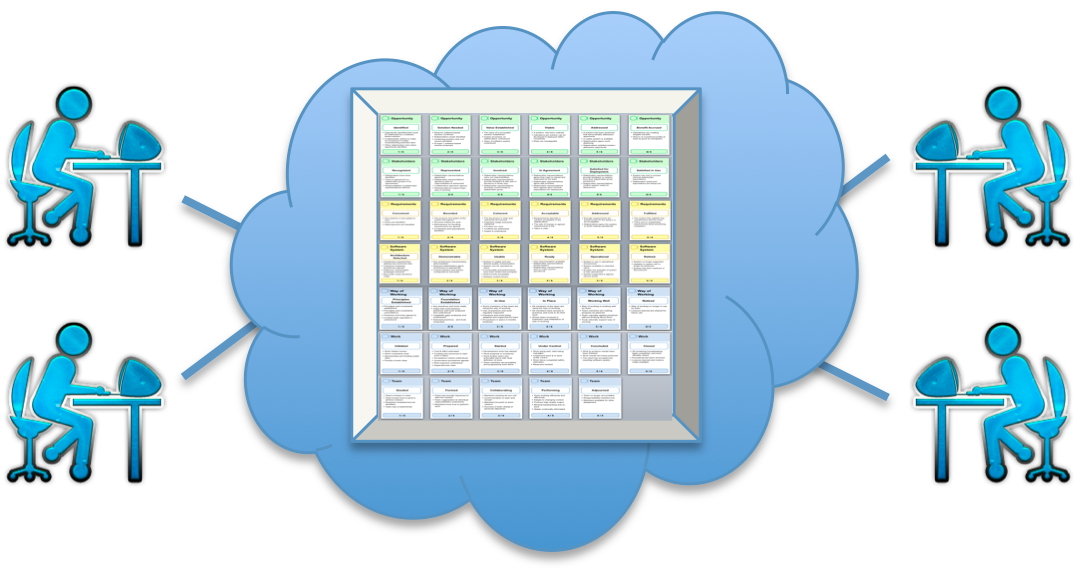
\includegraphics[width=3.40in]{project_steering_images/DigitalEssenceBoard.png}
\caption{Digital Essence board}
\label{DigitalEssenceBoard}
\end{figure}

After the initial presentation, the alphas were introduced incrementally over a number of 30 minute sessions, in order to make the experience as lightweight as possible. Each team met individually with a faculty and applied Essence on their practicum project. As an example, here is what happened with one team over a one-month period:

\underline{\textbf{Session 1}}: The two \quotes{customer} alphas, \textbf{Opportunity} and \textbf{Stakeholder}, were introduced. The main reason for introducing these two alphas first, was simply because it generally makes sense to have a discussion around the opportunity and stakeholders early in the project and before drilling down into the details of the solution and endeavor.

\underline{\textbf{Session 2}}: After updating the progress made for the previously introduced alphas, one \quotes{solution} alpha, \textbf{Requirements}, was introduced. The rationale for introducing this alpha was based on a pain point, as the team was expressing concerns around the client's expectations and hence needed to have a discussion around project scope and success criteria in relation with the \textbf{Requirements} alpha.

\underline{\textbf{Session 3}}: After updating the progress made for previously introduced alphas, two \quotes{endeavor} alphas, \textbf{Team} and \textbf{Way of Working}, were introduced based on additional pain points. Indeed the team was having some communication issues and hence needed to have a discussion around team collaboration and way of working.

\underline{\textbf{Session 4}}: After updating the progress made for previously introduced alphas, the remaining alphas were introduced for completeness: \textbf{Software System} and \textbf{Work}.

For each alpha, the team identified the current state, the target state, and any work items necessary to progress from the current to the target state. The identification of the current and target states was done through an informal discussion until the team reached an agreement.

To continue the example above, during the second session the team identified \textit{Conceived} as the current state for the \textbf{Requirements} alpha and \textit{Bounded} for the target state. Indeed all the items on the \textit{Conceived} checklist were satisfied while a few items on the Bounded checklist were not satisfied. In order to achieve \textit{Bounded}, the team first needed to define the project scope and clarify the success criteria with the client, as illustrated in Figure \ref{WorkItems}. The work items were dealt with right away or added to the team's work item list or backlog.

\begin{figure}[h]
\centering
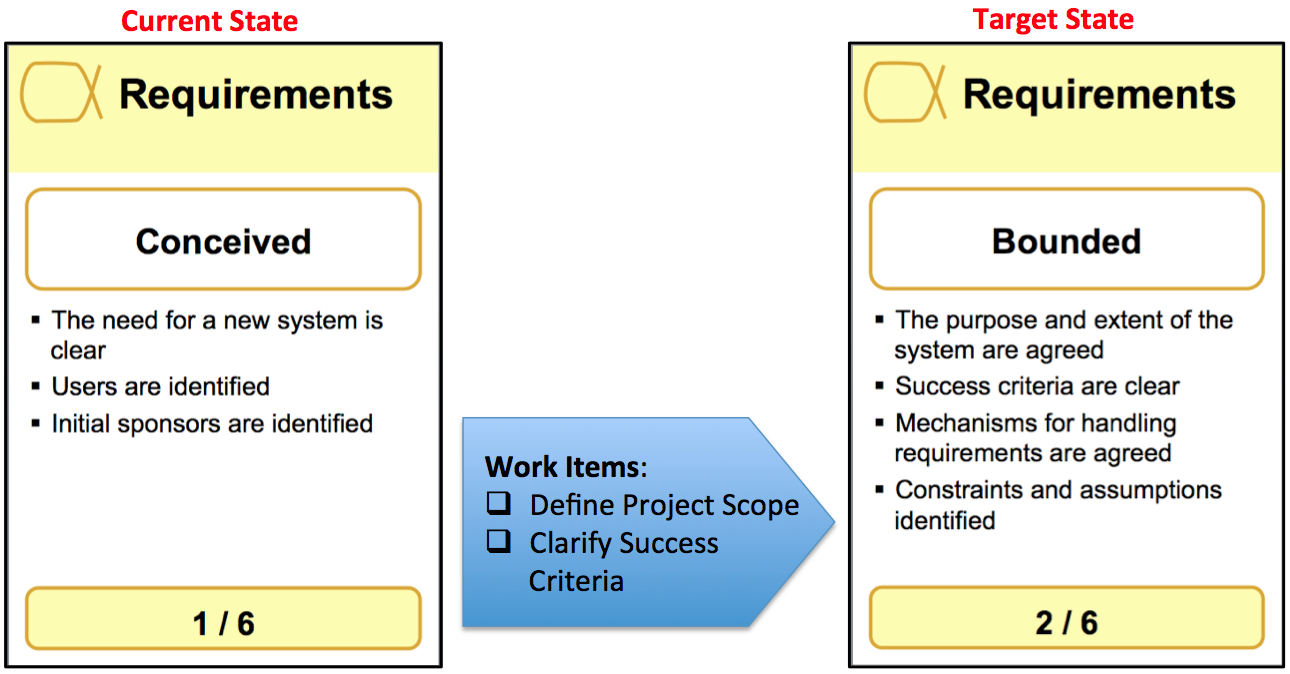
\includegraphics[width=3.30in]{project_steering_images/WorkItems.png}
\caption{Work items to reach the Bounded state}
\label{WorkItems}
\end{figure}

With mentoring from faculty, Essence was introduced to the geographically distributed teams using the incremental approach described above. For each team, and following the initial presentation of the Essence framework, four sessions of about 30 minutes long were necessary in order to introduce all the seven alphas incrementally. During each session, elements relevant to our study were jointly logged by students and faculty as described in Section \ref{UsingEssenceOnPracticumProjects} below.

\subsubsection{Second Pilot Projects - Workshop Approach}
In the Summer 2013 semester, Essence was introduced to four co-located teams at the beginning of the project. Based on our previous experience with the distributed students and armed with encouraging results (presented in Section \ref{FieldStudyAnalysis} below), we decided to speed-up the introduction process using a workshop approach. Our goal was to help the teams benefit from Essence as early as possible in the lifecycle.

The workshop was time-boxed to 90 minutes and included all students. It consisted of a general introduction of the Essence framework, the motivation for adopting the framework, together with exercises teaching each team how to apply the Essence's monitoring and steering approach on their own practicum project, one alpha at a time. Like in the first pilot projects and for the same reasons, the two green \quotes{customer} alphas, \textbf{Opportunity} and \textbf{Stakeholders}, were introduced first. Then, the remaining alphas (\textbf{Requirements}, \textbf{Software System}, \textbf{Team}, \textbf{Way of Working}, and \textbf{Work}) were introduced based on pain points when applicable, or in a random order otherwise. For each alpha, each team was tasked of identifying their project current state, target state, and any work items necessary to transition from the current to the target state. The identified work items were added to the team's work item list or backlog.

A couple of changes were introduced compared to the first pilot projects:

\begin{itemize}
    \item \textbf{Moving from physical cards to physical strips.} Handling a large set of cards could be a hassle. Therefore, we decided to create strips instead, as illustrated in Figure \ref{OneAlphaStrip}. For each alpha, one strip represents the typical sequence of states that the alpha progresses through during the project lifecycle. This way, we could easily provide the students with the information they needed to work on various alphas, one alpha at a time. Note that since the students were all physically present during the workshop, no digital boards were used.
    
    \item \textbf{Adoption of a poker game approach for state identification.} In order to remove anchoring bias, the informal way of identifying the current and target states was replaced with a \quotes{poker game} approach. In that context, each participant does a blind determination of their current state and all reveal their current state at the same time. In case of disagreement, the team discusses the different points of view until the participants reach an agreement. This technique is a simplification of Wideband Delphi \cite{StellmanAppliedPM} and agile estimation using Planning Poker \cite{GrenningPlanningPoker}, as the participants perform only one round of \quotes{estimation.} Just like Delphi and Planning Poker, the value is in the conversation, and allowing the team members to work through their different perspectives.
\end{itemize}

\begin{figure}[h]
\centering
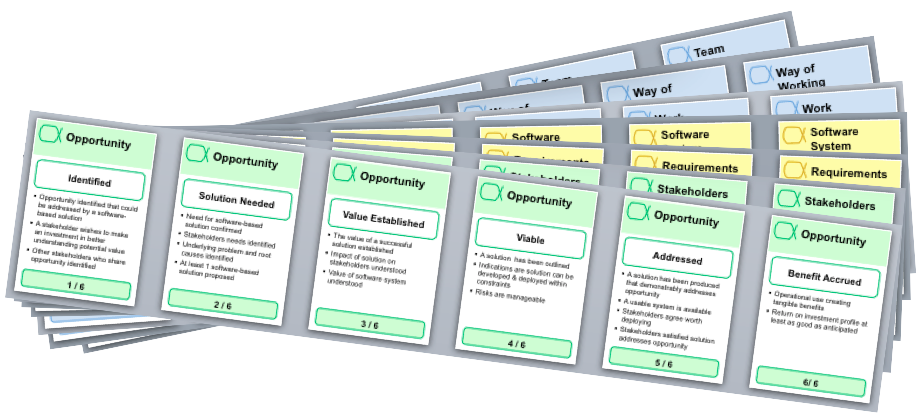
\includegraphics[width=3.30in]{project_steering_images/OneAlphaStrip.png}
\caption{One strip per alpha}
\label{OneAlphaStrip}
\end{figure}

Using the workshop approach described above, and with mentoring from faculty, Essence was introduced to the co-located teams over a 90 minutes session. On average, 10 minutes were necessary for a team to cover one alpha, and most teams were able to cover the seven alphas during the workshop. Students and faculty jointly logged elements relevant to our study as described in the following section.

\subsection{Using Essence on Practicum Projects}
\label{UsingEssenceOnPracticumProjects}
Once Essence was introduced, the teams were asked to continue leveraging the approach during the remainder of their project. Each team met on a regular basis (mostly weekly) for a 30 minutes session. During each session, the team reviewed most or all of the alphas. For each alpha, the team identified their project's current states following the poker game approach. The team would consider work items necessary to transition from the current state to the target state. Any new identified work items were added to the team's work item list or backlog. Teams were encouraged to act on their work items as soon as possible to accelerate their state progression

A faculty member was present to facilitate each session. Faculty involvement was kept at a minimum to limit influencing the steering of the project. The faculty's role was constrained to guiding the team through the application of the Essence monitoring and steering approach, and to validating the objectivity of the team's self-assessment of their project state. By listening to the team's discussions, and asking clarification questions as needed, the faculty gauged the project state. At times, this helped reduce the tendency of some teams to be overly pessimistic or optimistic about the project state.

For the purpose of the field study, progress and work items were recorded jointly by the students and faculty using the teams' Essence progress log, as shown in Table \ref{EssenceProgressLog}.

\begin{table*}[]
\centering
\caption{Essence progress log}
\renewcommand{\arraystretch}{1.4}
\label{EssenceProgressLog}
\begin{tabular}{|l|l|l|p{3.25in}|}
\hline
\multicolumn{4}{|l|}{Date:}                                         \\ \hline
\hline
Alpha           & Current State & Target State & Work Items / Notes \\
\hline
Stakeholders    &               &              &                    \\ \hline
Opportunity     &               &              &                    \\ \hline
Requirements    &               &              &                    \\ \hline
Software System &               &              &                    \\ \hline
Team            &               &              &                    \\ \hline
Way of Working  &               &              &                    \\ \hline
Work            &               &              &                    \\ \hline
\end{tabular}
\end{table*}

% \begin{figure}[h]
% \centering
% \includegraphics[width=3.30in]{project_steering_images/EssenceProgressLog.png}
% \caption{Essence progress log}
% \label{EssenceProgressLog}
% \end{figure}

The distributed students mostly used their digital Essence board, while the co-located teams used both digital Essence board and strips. Some students kept their strips handy and used them throughout the project lifecycle while others preferred to rely on the digital board.

At the end of the projects a survey was sent to the students, including the following questions:

\textbf{Survey Question 1}: What did you like the most about Essence? 

\textbf{Survey Question 2}: What did you like the least about Essence? 

\textbf{Survey Question 3}: In using Essence, did you adopt a practice that you wouldn't have? Or did you adopt it earlier than you would have without using Essence? (Please explain)

\textbf{Survey Question 4}: Was following the Essence approach worth your time? (Please explain why or why not)

\textbf{Survey Question 5}: Would you use Essence on your next project? (Please explain why or why not)

\textbf{Survey Question 6}: Anything else that we should know?

\section{FIELD STUDY ANALYSIS \& INTERPRETATION}
\label{FieldStudyAnalysis}
Our research questions relate to the value provided by the SEMAT Essence's monitoring and steering approach. The researchers measured the qualitative value based on students' feedback collected mostly during the weekly SEMAT sessions, course reflection reports, and final survey. The researchers measured the quantitative value based on alpha state progression as well as the number of work items generated during the weekly SEMAT sessions and allowing bringing the project to a higher state. Refer to Figure \ref{FieldStudyRowData} in the Appendix for the raw data collected on alpha state progression, and to Figure \ref{NewWorkItemsGenerated} under Research Question 3 for the number of work items generated by the approach per week.

\textbf{Research Question 1}: Does the SEMAT Essence's monitoring and steering approach provide value to the project team?

Our field study shows that students receive value from SEMAT Essence's monitoring and steering approach provided by the kernel alphas and their states. In our survey, 90\% of the students said that following the approach was worth their time (80\% of the students participated in the survey.) Similarly, 80\% said that they will use the approach on their next project.

By following the approach, project teams monitored their progression through the Essence states over time, as illustrated in Figure \ref{AlphaProgressionColocated4} for team Co-located-4. Every week this team generated on average 6 new work items during their SEMAT session, and then acted on these work items in order to bring the project to a higher state.

\begin{figure}[h]
\centering
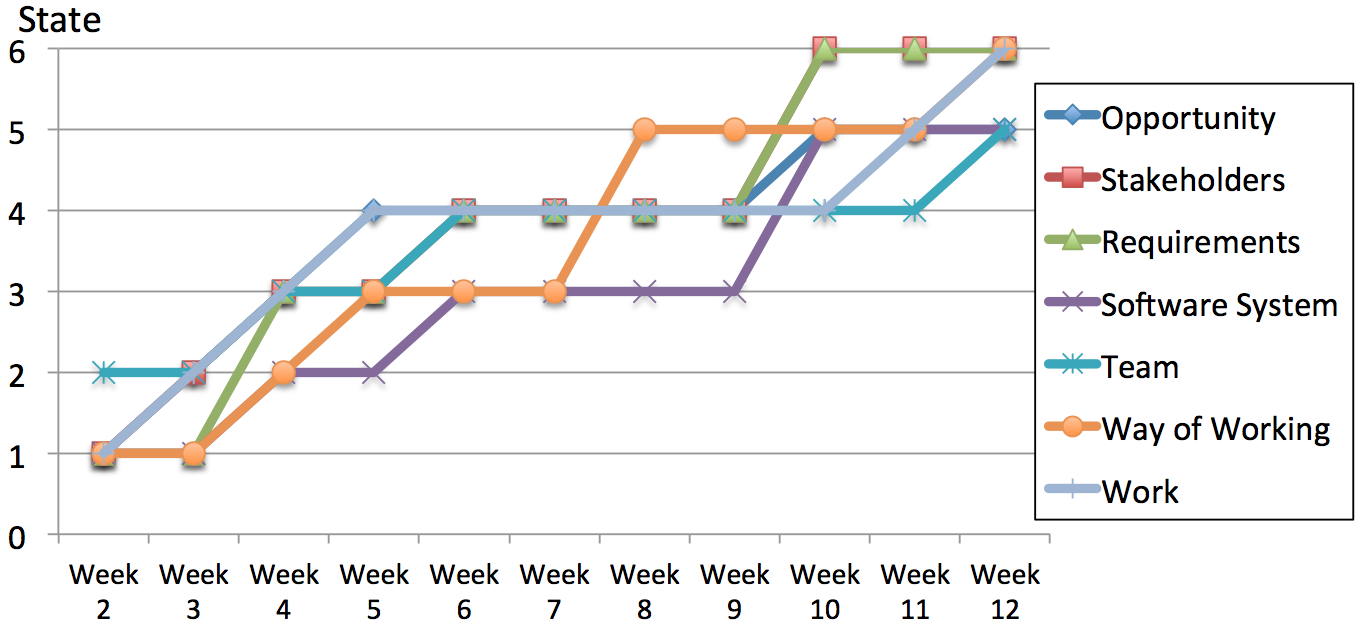
\includegraphics[width=3.30in]{project_steering_images/AlphaProgressionColocated4.png}
\caption{Alpha progression for team Co-located-4}
\label{AlphaProgressionColocated4}
\end{figure}


In conclusion, most students have a positive perception of this approach as it helps them make decisions allowing to move their project forward.

\textbf{Research Question 2}: How does SEMAT Essence's monitoring and steering approach provide value to the project team?

The benefits that a project team receives from SEMAT Essence's monitoring and steering approach come primarily from the discussions that occur when the team is covering the various alphas. The discussions enable the team to pause and assess the situation:

\begin{itemize}
    \item \textbf{The team steps back from its daily tasks and examines its project holistically.} One student noted: \participantQuote{Essence gives us a chance to step back and look at the project as a whole, from a bird's-eye view. There are aspects that we tend to ignore when focused on the technology. Essence is very useful, because it makes me think about these particular aspects.} Similarly, another student noted: \participantQuote{I like the fact that Essence provides a structured way of thinking about critical aspects of the project at different stages of the project. Without Essence, our team could have overlooked some of these aspects.} Stepping back and looking at the project holistically is a healthy exercise providing the distance and perspectives needed to understand a situation, reflect, and make decisions. When asked about what they like the most about Essence, most students mentioned reflection or retrospective. For instance one student noted: \participantQuote{Though the team was holding retrospectives every week already, having Essence discussions be a part of it allowed the team to touch on important aspects of the project.}
    
    \item \textbf{The team records progress accomplished and identifies what remains to be done.} When asked about what she liked the most about Essence, one student answered: \participantQuote{The choice of alphas: they seem to be exactly the right areas to monitor to promote the success of a software project.} The Essence mechanism for monitoring progress is illustrated in Figure \ref{ProjectStateDistributed3}. The chart shows the progress made by team Distributed-3 at week 5, compared to the practicum target state established by faculty. The team has been making good progress towards the target goal in most dimensions except \textbf{Software System} that lags at state 1 (\quotes{\textit{Architecture Selected}}). This situation served as a red flag and a reminder that the team needed to focus its effort on taking their software system to the next level. The approach was used as a similar risk management mechanism in other instances. When asked if he would use Essence on his next project, one student answered: \participantQuote{Yes, it 's great for team reflection and risk management.}
    
    \item \textbf{The team seeks guidance on what directions to take and identifies goals to transition to a higher project state.} Team Distributed-1 noted: \participantQuote{Essence gives us structure and direction.} Another student commented: \participantQuote{Essence is useful, as it gives you an agenda or checklist based on various dimensions (even though I was skeptical at first).} Essence provides a simple project steering mechanism. For each alpha, the identified target state provides the direction to take, and its checklist provides goals to reach. For instance and to continue the example above, during week 5 team Distributed-3 identified \quotes{\textit{Demonstrated}} as its target state for \textbf{Software System}, with a number of goals including demonstrating the key architecture characteristics, as illustrated in Figure \ref{ProjectStateDistributed3}.
    
    \item \textbf{The team decides what to do to reach the target goals. Once the team identifies the goals, the team members rely on their software engineering knowledge and experience to decide how to reach these goals.} Indeed, Essence does not prescribe the use of any existing method (like Scrum or XP) or set of practices or work items. Instead, the team has the flexibility to leverage any method or set of practices that best suit their needs, and decide what work items to perform to reach the goals set by the target state. As a consequence, our seven practicum teams were able to leverage Essence even though they all used a different set of software engineering practices. When asked if he would use Essence on his next project, one student answered: \participantQuote{Yes, especially with a project team that is not used to the same software engineering process. In that instance Essence is a backdrop at the basis of the communication about all the considerations for the success of the project.} Another student added: \participantQuote{It is simple, lightweight and useful.}
\end{itemize}

\begin{figure}[t]
\centering
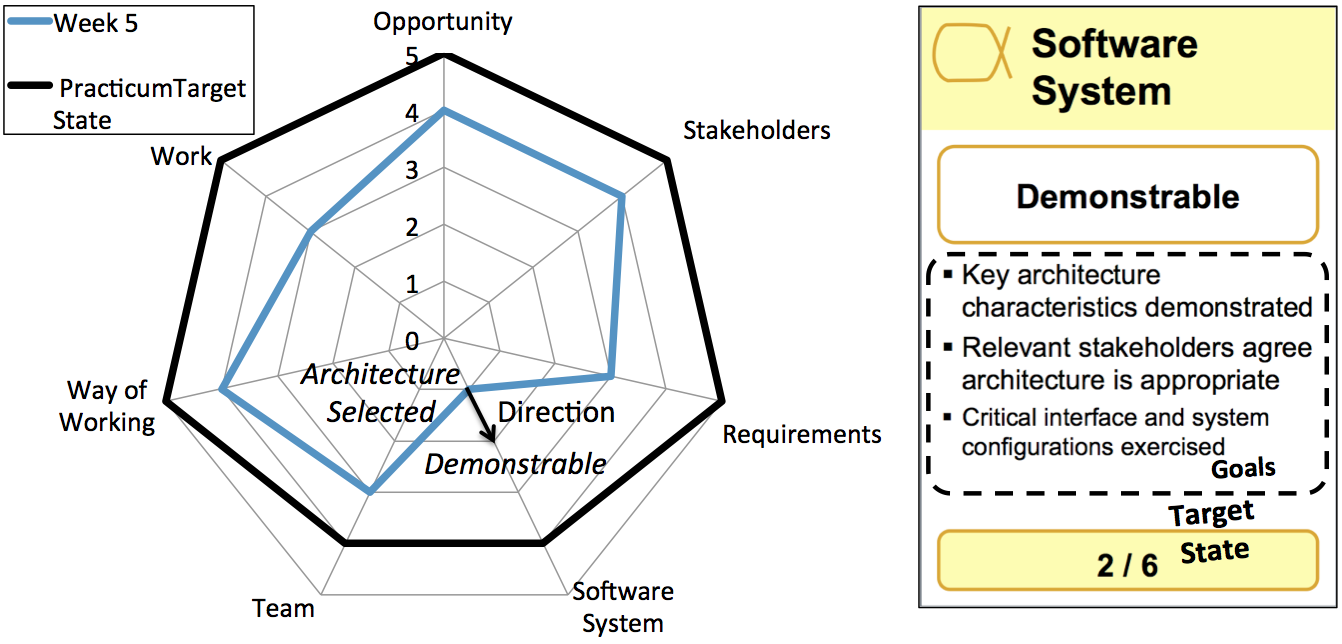
\includegraphics[width=3.30in]{project_steering_images/ProjectStateDistributed3.png}
\caption{Project state for team Distributed-3 at week 5, with direction and goals for Software System}
\label{ProjectStateDistributed3}
\end{figure}


The team accelerates its state progression by acting on its work items as soon as possible and iterating through the steps described above. Figure \ref{EssenceMonitoringLoop} illustrates this iterative process.

\begin{figure}[t]
\centering
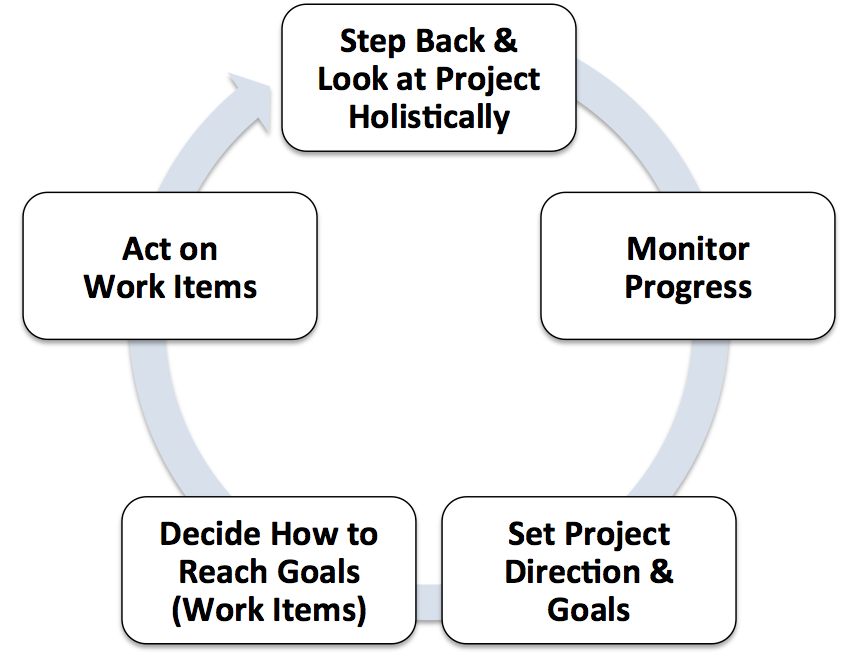
\includegraphics[width=3.30in]{project_steering_images/EssenceMonitoringLoop.png}
\caption{Essence monitoring and steering loop}
\label{EssenceMonitoringLoop}
\end{figure}

In answer to our second research question, the approach adds value by providing the project team with a holistic view of the project, a mechanism for monitoring progress and steering projects, as well as an effective structure for team reflection and risk management. This is provided in a simple, lightweight, non-prescriptive and method-agnostic fashion.

\textbf{Research Question 3}: When in the project lifecycle does the SEMAT Essence's monitoring and steering approach add value?
The value that the teams receive from SEMAT Essence's monitoring and steering approach varies over the project lifecycle. Our study shows that most value is generated at the beginning of the project and that it decreases thereafter. Here are some illustrating quotes:
\begin{itemize}
    \item When asked if following the Essence approach was worth their time, 20\% of the students who answered yes to the question qualified their answers as follows: \participantQuote{Yes, it helped us at the beginning of the project}, or \participantQuote{Yes, it was worth my time in the first half of the project.}
    
    \item Among the students who mentioned that they would use Essence on their next project, one qualified her answer as follows: \participantQuote{Yes, but only at the beginning of the project.}
    
    \item When asked what he liked the least about Essence, one student answered: \participantQuote{Essence lost value once the project settled because we dead ended on a set of cards.} Another student added: \participantQuote{Essence is useful in the planning stages. Later on its usefulness is dying down. If you spend multiple weeks on one card, then spending time looking at it is less helpful.} This opinion is shared by about 50\% of the students.
    
    \item The faculty in charge of the practicum course, and who has taught the course for 10 years, noted: \participantQuote{Compared to previous years, I see a much better early project organization with lot less floundering. I hope that we keep using Essence in the future. We should definitely keep it at the beginning of the projects.}
\end{itemize}

The alpha progression of team Co-located-3 illustrates the decrease in value, as seen in Figure \ref{AlphaProgressionColocated3}. The chart shows that the team progresses well during the first half of the project, then reaches a plateau or stable state during a few weeks, before progressing again at the end of the project. This picture represents most teams' progressions.

\begin{figure}[t]
\centering
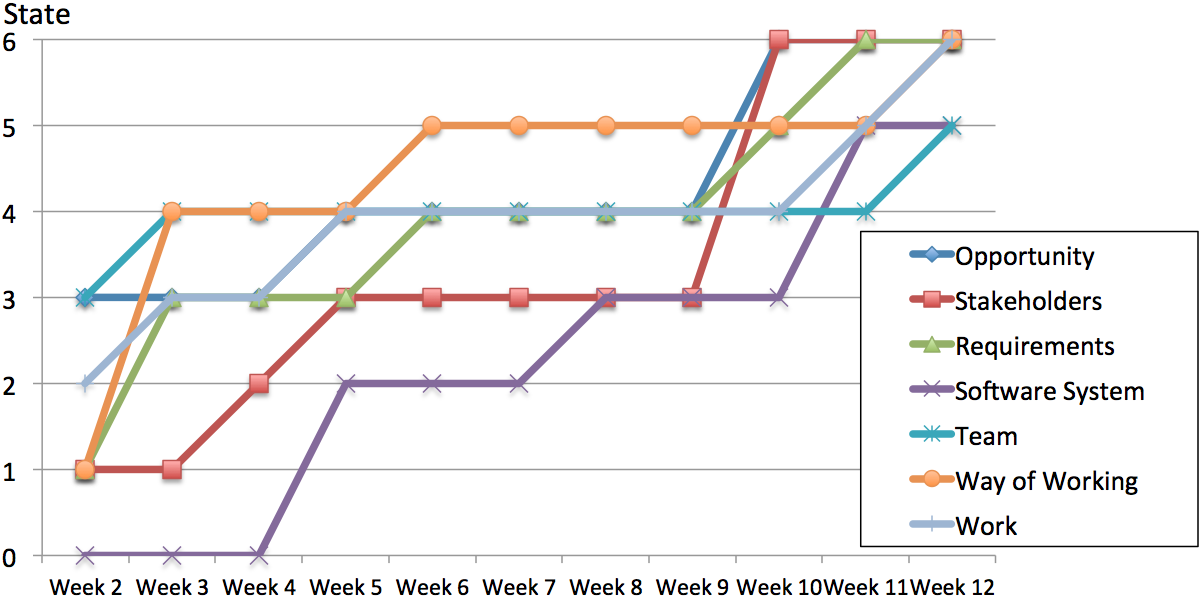
\includegraphics[width=3.30in]{project_steering_images/AlphaProgressionColocated3.png}
\caption{Alpha progression for team Co-located-3}
\label{AlphaProgressionColocated3}
\end{figure}


By analyzing the work items generated by the team during the weekly SEMAT sessions, we find that the initial progression in Figure \ref{AlphaProgressionColocated3} is driven by those work items. Indeed these work items significantly contribute to bringing the project to a higher state. However, the final progression is done independently of Essence as the approach generates few work items at the end of the project. Most teams experienced this phenomenon, as illustrated in Figure \ref{NewWorkItemsGenerated} showing a consistent drop of work items over time.

\begin{figure}[t]
\centering
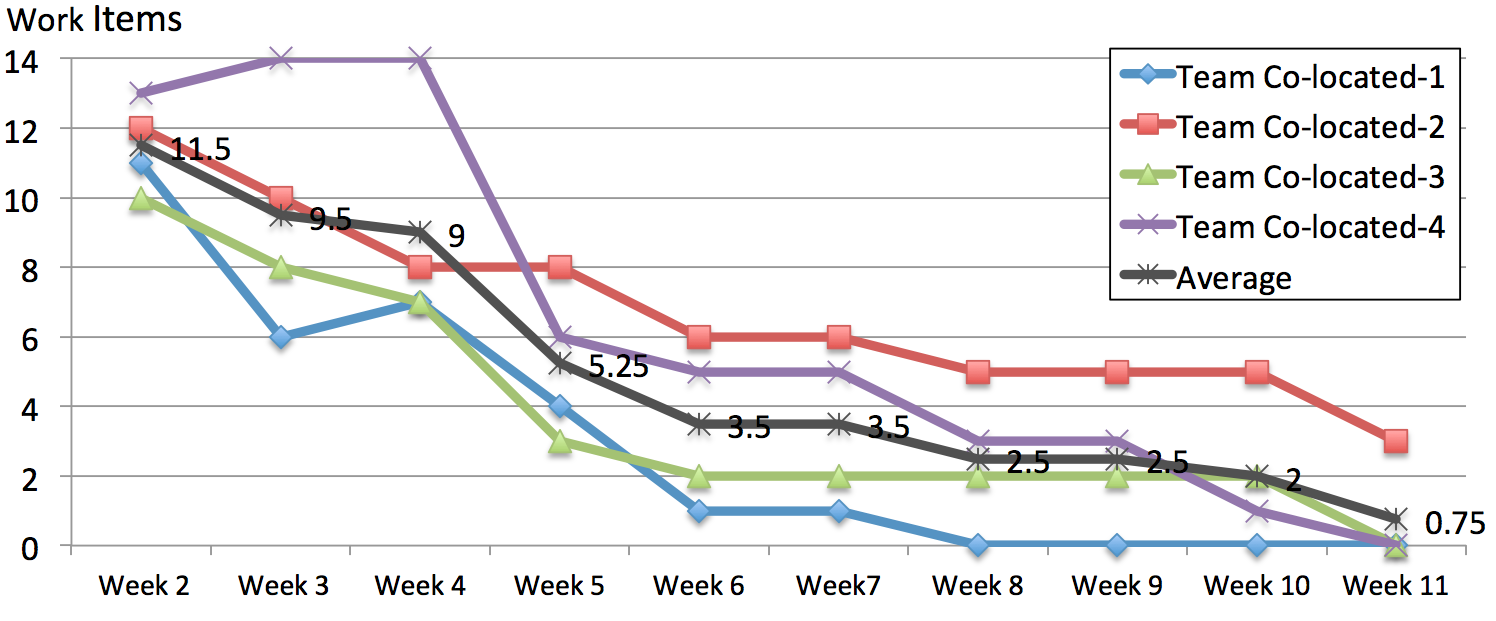
\includegraphics[width=3.30in]{project_steering_images/NewWorkItemsGenerated.png}
\caption{New work items generated per week}
\label{NewWorkItemsGenerated}
\end{figure}

Despite the value decrease, the students' perception of the approach remains positive by the end of the project according to the survey responses. Indeed a majority of students answered without qualification that they found Essence worth their time and will use the approach on their next project. A majority of students also mentioned reflection or retrospective as a strength of the approach. One student mentioned: \participantQuote{Even though we are not generating new tasks, the [SEMAT] meetings remain useful as they give us the opportunity to reflect upon our project.} Similarly, team Distributed-1 noted in its reflection report: \participantQuote{The team was pleased to see that Essence covered `The Way of Working' as well as ‘The Team'. These two topics generated useful team introspection at the beginning of the practicum and were nice reminders that the team does constant checkups for the overall condition of the members and the project.}

In conclusion, the SEMAT Essence's monitoring and steering approach provided by the kernel alphas and their states is most effective at the beginning of the project. The effectiveness decreases over time. Indeed, the approach gradually loses its ability to enable the team to steer the project by generating new work items leading to a higher project state. The reasons behind the value decrease are explored in the next research question. However, most teams continue to perceive value throughout the lifecycle out of the approach reflection mechanism.

\textbf{Research Question 4}: What are the limitations to the approach's effectiveness?

The previous section shows that the effectiveness of the approach decreases over time. This phenomenon could be explained by a number of factors. One factor relates to the fact that the need for the approach varies throughout the project lifecycle. For instance, as the project team matures and becomes a high-performing team producing high quality outcome, it becomes a self-steering team requiring less support from the approach. Similarly, once most project risks have been mitigated, the team requires less risk management support. Therefore, unless there is a disruptive event reverting the project to a lower state, the value decrease is to be expected.

In addition, some kernel characteristics influence the value decrease. Most Essence alphas have more states supporting the progression through the initial project phase compared to later phases. Figure \ref{NumberOfAlphaStatesPerRUPPhase} illustrates this phenomenon using the RUP \cite{KrollRUP} phases (Inception, Elaboration, Construction, and Transition) as an example. The chart shows that for most alphas, the number of states per phase is higher in Inception compared to the other phases. For five out of seven alphas, there is only one state in Construction. Most project teams spend the majority of their time in Construction. As a result, for these alphas the teams end-up remaining in the same state during their entire Construction phase. This lack of alpha states covering the Construction phase might be due to the fact that most of the technical work done in Construction is practice-specific, and therefore not supported by the universal kernel. Further investigations are necessary to identify potential ways to extend the kernel so it better supports the work done during Construction.

\begin{figure}[t]
\centering
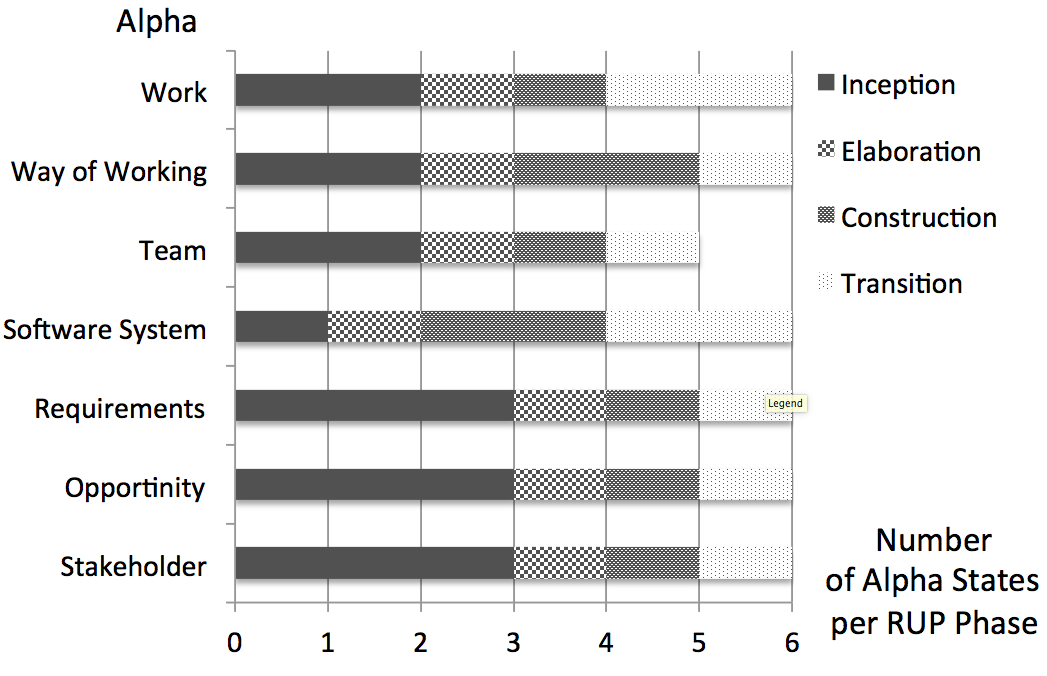
\includegraphics[width=3.30in]{project_steering_images/NumberOfAlphaStatesPerRUPPhase.png}
\caption{Number of alpha states per RUP phase}
\label{NumberOfAlphaStatesPerRUPPhase}
\end{figure}

By definition, the Essence kernel is geared towards steering a project or release throughout its entire lifecycle in a fairly linear fashion dictated by the alpha state progression. By repeating through the Essence monitoring and steering loop (see Figure \ref{EssenceMonitoringLoop}), the team steers the project or release through the sequence of states for each alpha. This process is designed to support the work done at the release level and not to support the work done at the iteration level because of the following reasons:

\begin{itemize}
    \item The kernel is lifecycle-independent and therefore does not provide specific support for iterative development.
    
    \item The kernel alpha states and their checklist items are specified at the project or release level, not at the iteration level.
\end{itemize}

Consequently, we were unable to effectively leverage the approach to help steer projects during Construction on iterative projects. The teams received some guidance on iterative development from whatever method they adopted, like Scrum and XP that are optimized for iterative development.

In conclusion, the observed value decrease could be explained by three factors. The first factor is a decrease in the need for the approach as the team matures and becomes self-steering. The second factor is a front-end focus of the alphas, making the approach most effective during project initiation. The third factor relates to the definition of the kernel alpha checklists, which are specified at the project or release level, not at the iteration level. This explains the value decrease during construction on iterative projects.

As a result, the monitoring and steering mechanisms are most effective during project initiation and for monitoring and steering the work done at the project or release level. This type of work could be qualified as \quotes{universal} as it is generally common across projects. This confirms that the kernel provides effective support for universal work. Support for non-universal technical work has to come from additional practices added on top of the kernel, or by extending or altering the kernel definition.

Finally, a limitation pointed out by about 40\% of the students in the survey, is related to some ambiguity in the alpha checklists definition. For instance, one student mentioned: \participantQuote{The checklist within an alpha can have cryptic language. Sometime, the points are ambiguous.} Here are some examples of typical student reactions:

\textbf{Checklist Item}: Enough of the requirements are addressed \ldots 

\textbf{Student}: \participantQuote{What do they mean by `enough'?}

\textbf{Checklist Item}: Constraints are identified and considered. 

\textbf{Student}: \participantQuote{What kind of constraints are they talking about?}

\textbf{Checklist item}: Critical interfaces have been demonstrated. 

\textbf{Student}: \participantQuote{What do they mean by `demonstrated'?}

\textbf{Checklist Item}: The key practices and tools that form the foundation of the way-of-working are selected.

\textbf{Student}: \participantQuote{Which tools form the foundation of the way-of-working?}

Thus, a limitation to the approach effectiveness comes from some ambiguities in the alpha checklist definitions, leading to situations where the team discusses the meaning of a checklist item instead of having a conversation about the project. At times, this disrupts the flow of otherwise valuable team discussions.

\section{FROM THE EDUCATOR'S PERSPECTIVE}
This section shares some of our findings related to introducing Essence to a project team having no prior experience with the approach, together with a few words of caution related to the use or misuse of Essence for evaluation purposes.

\subsection{Incremental versus Workshop Introduction Approaches}

Our experience with both the incremental and workshop approaches to introducing Essence indicates that both have value and that adoption resistance drives which approach is best for the situation.

\subsubsection{Incremental}
The incremental introduction approach brings immediate value to the teams, as noted by team Distributed-2 in its reflection report: \participantQuote{The team found Essence valuable right from the start. [...] it helped manage the direction and organization of the team by examining overlooked aspects of the project.} For instance, during the first session, this team identified the work items \quotes{Understand the risks and constraints} and \quotes{Identify all stakeholders} based on its discussion around the \textbf{Opportunity} alpha and \textbf{Stakeholder} alpha respectively. Some previous practicum teams overlooked these kinds of discussions and work items. However, this approach delays many important conversations until all the alphas are introduced.

This approach has minimum perceived overhead. In our case, introducing Essence incrementally required only a weekly session of 30 minutes, during a five weeks period.

When adoption resistance might be an issue, we recommend introducing the approach incrementally through a series of regular (e.g. weekly) and short (e.g. 30 minutes) sessions. We also recommend having one dedicated faculty or coach per team.

\subsubsection{Workshop}
The workshop introduction approach introduces all the alphas at once, hence enabling the team to look at its project holistically while having conversations covering the various project's dimensions as early as possible.

This approach requires that each team invest in one upfront workshop during which the team starts applying Essence directly to its current project. During our 90 minutes introduction workshop, 10 minutes were needed to set the context and motivate the exercise. The remaining 80 minutes was enough time for most teams to have a substantial conversation about their perception of the project's current state and to generate work items to make forward progress. On average, 10 minutes were necessary for a team to cover one alpha, and most teams were able to cover the seven alphas during the workshop. However, our largest team of five members took an average of 20 minutes per alpha and hence had to complete the exercise during a follow-up session. The size of the team as well as internal disagreements generated some longer conversations.

We recommend adjusting the workshop duration based on the team size and any other known parameters that might influence the length of the conversations, like team dynamic or project uncertainty. We also recommend having one dedicated faculty or coach per team.

Table \ref{ComparingWorkshopAppoaches} summarizes and compares the incremental and workshop introduction approaches. We recommend the workshop approach when introducing Essence, unless faced with initial adoption resistance that may require a slower incremental approach.

\begin{table}[]
\centering
\renewcommand{\arraystretch}{1.4}
\caption{Comparison of introduction approaches}
\label{ComparingWorkshopAppoaches}
\begin{tabular}{|p{0.6in}|p{1.1in}|p{1.1in}|}
\hline
Approach      & Incremental                                                                 & Workshop  \\
\hline
Description   & Essence alphas are introduced incrementally over a number of short sessions & Essence alphas are introduced all at once during a single session \\
\hline
Benefits      & Brings immediate value with minimum overhead                                & Brings immediate and optimum value (all alphas are covered)       \\
\hline
Drawbacks     & Full benefit is delayed until complete introduction of alphas               & Requires initial overhead                                         \\
\hline
When to Apply & In case of adoption resistance                                              & Always, except in case of adoption resistance  \\                  
\hline
\end{tabular}
\end{table}

Given our recommendation of one faculty per team, in the future, we plan on introducing Essence and conducting a full assessment during a 90-minute team meeting. In a course with five teams, scheduling five separate team meetings is easier than trying to do five simultaneous team meetings with five instructors.

Following the introduction of Essence, we recommend that each project team continue to meet on a regular (e.g. weekly) basis for a short (e.g. 30 minutes) session throughout the initial project phase. Once a team reaches \quotes{construction} and becomes a high-performing team producing high quality outcome, the frequency of the sessions could decrease because the team needs less support from the approach.

\subsection{Alpha Introduction Order}
Participants can be overwhelmed when shown all the states for all the alphas at once. Introducing the alphas one at a time solves this problem, whether this is done incrementally over a series of meetings or during a single session or workshop.

We recommend introducing the \textbf{Stakeholder} and \textbf{Opportunity} alphas (aka the customer dimension) first, since it generally makes sense to have a discussion around this dimension before drilling down into the details of the solution and endeavor. We introduce \textbf{Stakeholder} prior to \textbf{Opportunity} since many participants find it easier to relate to the \textbf{Stakeholder} alpha than the abstract \textbf{Opportunity} alpha. The other alphas could be introduced as needed based on pain points. When in doubt about which alpha to introduce next, one alpha could be selected randomly. Indeed, the value is in having a holistic view of the project, therefore looking at any dimension has potential benefits.

\subsection{A Word of Caution}
As noted by William Cameron \cite{CameronSociologicalThinking}, \quotes{not everything that can be counted counts, and not everything that counts can be counted.} This is especially true when it comes to individual and team performance evaluation, where using metrics could be dangerous. Inappropriate metrics could be used (like measuring a developer performance based on the number of lines of code produced), metrics could be gamed, and metrics do not give the full picture.

As an example, Figure \ref{AvoidThisKindOfComparison} shows the final state of our distributed teams at the end of their project. From the chart, one might infer that Team Distributed-3 outperformed Team Distributed-1, which in turn outperformed Team Distributed-2 that lagged behind. In fact, despite having the highest project state, Team Distributed-3's work was slightly disappointing according to both the clients and faculty. The team ended-up with a lower grade compared to the other teams. This was due to quality issues during various product demonstrations and a lack of architecture documentation that surfaced during the team final presentation. This makes the team self-assessment of the \textbf{Software System} alpha and therefore of its overall project state questionable. Team Distributed-2 lagged only behind because the initial solution proposed by the client turned out to be infeasible, and the team did an excellent job redirecting the project into a constructive direction and hence earned an excellent grade. The routinely low \textbf{Software System} alpha state served as a red flag for risk management purposes, not evaluation purposes.

\begin{figure}[t]
\centering
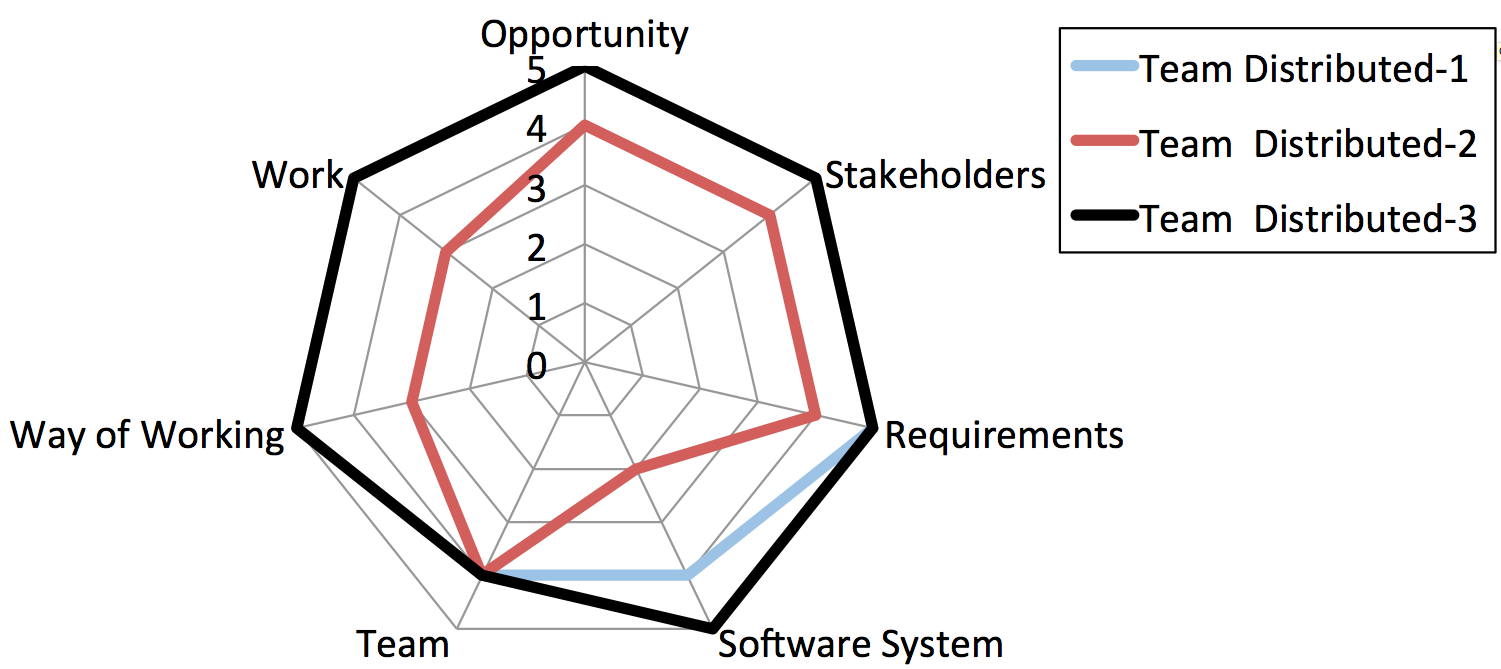
\includegraphics[width=3.30in]{project_steering_images/AvoidThisKindOfComparison.png}
\caption{Final project state of the distributed teams: Avoid this kind of comparison}
\label{AvoidThisKindOfComparison}
\end{figure}


In conclusion, we recommend leveraging the approach to identify projects at risk rather than for performance evaluation purposes. Some teams might be only ahead because they are overly optimistic about their project state, while others might be behind because of circumstances beyond their control.

\section{CONCLUSION}
This paper presents the results of a field study aiming at understanding the value project teams receive from following the SEMAT Essence's monitoring and steering approach provided by the Essence kernel alphas and their states. The study involved seven teams of master students with no prior knowledge of Essence.

The study validated our research hypothesis by showing that the approach provides student teams with a simple, lightweight, non-prescriptive and method-agnostic way to examine their projects holistically, structure team reflections, manage risks, monitor progress and steer their projects. Compared to the ten previous years, the faculty in charge of the practicum course noted that there was \participantQuote{much better early project organization with a lot less floundering.} Indeed, the approach enables students to learn to steer projects effectively by addressing the various dimensions of software engineering.

The study also highlighted that the monitoring and steering mechanisms are most effective during project initiation and for monitoring and steering the work done at the project or release level. This type of work could be qualified as \quotes{universal} as it is generally common across projects. This confirms that the kernel provides an effective support for universal work. Support for non-universal technical work should come from additional practices added on top of the kernel, or by extending or altering the kernel definition.

The results of this paper are limited to evaluating the effectiveness of the Essence approach when a facilitator is involved. Even though faculty involvement was kept at a minimum to limit influencing the students, a faculty served as facilitator during the SEMAT meetings throughout the practicum projects. More research is necessary to assess the effectiveness of the approach without facilitators.

The project context was fairly similar for all teams, except for their geographic distribution and average work experience. While the study has not revealed any influences of these contextual factors on the approach's effectiveness, additional data is required to confirm or refute any impact. The Essence steering and monitoring approach appears equally applicable to both co-located and geographically distributed teams.

We are currently working with another set of practicum teams at Carnegie Mellon University in Silicon Valley to gather more data necessary to evaluate the SEMAT Essence's monitoring and steering approach, with a focus on both effectiveness of the approach and accuracy of the model.

\section{ACKNOWLEDGMENTS}
We would like to acknowledge the contributions of all the reviewers, and thank them for their insightful comments on early drafts of this paper. A special thanks to Hakan Erdogmus and Maria Nelson for their thorough reviews and invaluable suggestions, and to Ed Katz for recommending that we conduct our field study in the context of his practicum course and for his support throughout the study. Finally, we would like to warmly thank the students who participated in the study, for their openness and insights.

\section{APPENDIX}
Figure \ref{FieldStudyRowData} below provides the reader with the field study row data on alpha state progression. Each number in bold (from 1 to 6) represents an alpha state. Each number in italic (from 2 to 15) represents the week during which the team reaches the state. For instance, team Distributed-1 reaches the \textbf{Stakeholder} state 1 at week 2. Two or more italic numbers in one cell reflects a state backtracking. For instance, team Co-located 2 reaches the \textbf{Team} state 3 at week 2. The team then progresses to a higher state, but backtracks to state 3 at week 10.

\begin{figure*}[h]
\centering
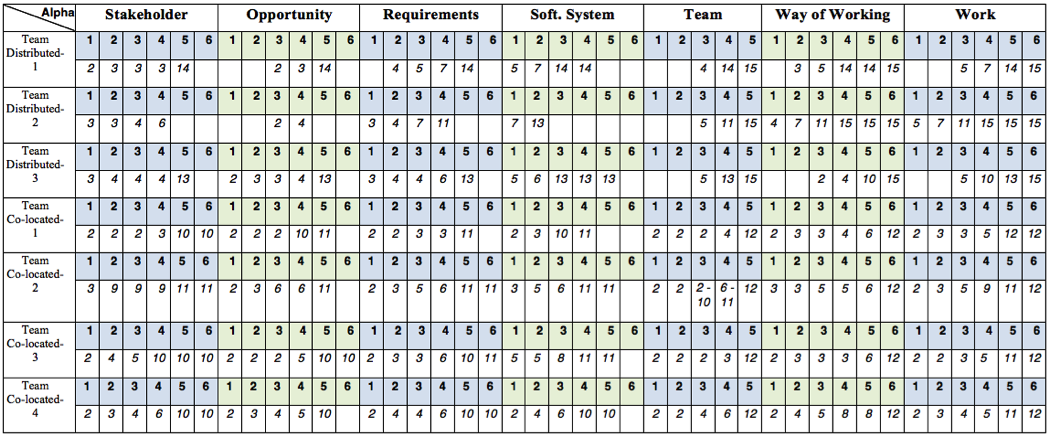
\includegraphics[width=6.80in]{project_steering_images/FieldStudyRowData.png}
\caption{Field study row data on alpha state progression}
\label{FieldStudyRowData}
\end{figure*}


% \begin{table*}[]
% \centering
% \renewcommand{\arraystretch}{1.3}
% \caption{Field study row data on alpha state progression}
% \label{FieldStudyRowDatal}
% \begin{tabular}{|l|l|l|l|l|l|l|l|l|l|l|l|l|l|l|l|l|l|l|}
% \hline
%                   & \multicolumn{6}{l|}{Stakeholders} & \multicolumn{6}{l|}{Opportunity} & \multicolumn{6}{l|}{Requirements} \\ \hline
%                   & 1   & 2   & 3   & 4   & 5   & 6   & 1   & 2   & 3  & 4   & 5   & 6   & 1   & 2   & 3   & 4   & 5   & 6   \\ \hline
% Team Distributed-1 & 2   & 3   & 3   & 3   & 14  &     &     &     & 2  & 3   & 14  &     &     & 4   & 5   & 7   & 14  &     \\ \hline
% Team Distributed-2 & 3   & 3   & 4   & 6   &     &     &     &     & 2  & 4   &     &     & 3   & 4   & 7   & 11  &     &     \\ \hline
% Team Distributed-3 & 3   & 4   & 4   & 4   & 13  &     & 2   & 3   & 3  & 4   & 13  &     & 3   & 4   & 4   & 6   & 13  &     \\ \hline
% Team Co-located-1  & 2   & 2   & 2   & 3   & 10  & 10  & 2   & 2   & 2  & 10  & 11  &     & 2   & 2   & 3   & 3   & 11  &     \\ \hline
% Team Co-located-2  & 3   & 9   & 9   & 9   & 10  & 11  & 2   & 3   & 6  & 6   & 11  &     & 2   & 3   & 5   & 6   & 11  & 11  \\ \hline
% Team Co-located-3  & 2   & 4   & 5   & 10  & 10  & 10  & 2   & 2   & 2  & 5   & 10  & 10  & 2   & 3   & 3   & 6   & 10  & 11  \\ \hline
% Team Co-located-4  & 2   & 3   & 4   & 6   & 10  & 10  & 2   & 3   & 4  & 5   & 10  &     & 2   & 4   & 4   & 6   & 10  & 10  \\ \hline
% \end{tabular}
% \end{table*}


% \begin{table*}[]
% \centering
% \caption{My caption}
% \label{my-label}
% \begin{tabular}{|l|l|l|l|l|l|l|l|l|l|l|l|l|l|l|l|l|l|l|l|l|l|l|l|l|l|l|l|l|l|l|l|l|l|l|l|l|l|l|l|l|l|}
% \hline
%                   & \multicolumn{6}{l|}{Stakeholders} & \multicolumn{6}{l|}{Opportunity} & \multicolumn{6}{l|}{Requirements} & \multicolumn{6}{l|}{Software System} & \multicolumn{5}{l|}{Team} & \multicolumn{6}{l|}{Way of Working} & \multicolumn{6}{l|}{Work} \\ \hline
%                   & 1   & 2   & 3   & 4   & 5   & 6   & 1   & 2   & 3  & 4   & 5   & 6   & 1   & 2   & 3   & 4   & 5   & 6   & 1    & 2   & 3    & 4    & 5   & 6   & 1   & 2  & 3  & 4   & 5   & 1   & 2   & 3   & 4    & 5    & 6   & 1  & 2  & 3 & 4 & 5  & 6  \\ \hline
% Team Distributed-1 & 2   & 3   & 3   & 3   & 14  &     &     &     & 2  & 3   & 14  &     &     & 4   & 5   & 7   & 14  &     & 5    & 7   & 14   & 14   &     &     &     &    & 4  & 14  & 15  &     & 3   & 5   & 14   & 14   & 15  &    &    & 5 & 7 & 14 & 15 \\ \hline
% Team Distributed-2 & 3   & 3   & 4   & 6   &     &     &     &     & 2  & 4   &     &     & 3   & 4   & 7   & 11  &     &     &      &     &      &      &     &     &     &    &    &     &     &     &     &     &      &      &     &    &    &   &   &    &    \\ \hline
% Team Distributed-3 & 3   & 4   & 4   & 4   & 13  &     & 2   & 3   & 3  & 4   & 13  &     & 3   & 4   & 4   & 6   & 13  &     &      &     &      &      &     &     &     &    &    &     &     &     &     &     &      &      &     &    &    &   &   &    &    \\ \hline
% Team Co-located-1  & 2   & 2   & 2   & 3   & 10  & 10  & 2   & 2   & 2  & 10  & 11  &     & 2   & 2   & 3   & 3   & 11  &     &      &     &      &      &     &     &     &    &    &     &     &     &     &     &      &      &     &    &    &   &   &    &    \\ \hline
% Team Co-located-2  & 3   & 9   & 9   & 9   & 10  & 11  & 2   & 3   & 6  & 6   & 11  &     & 2   & 3   & 5   & 6   & 11  & 11  &      &     &      &      &     &     &     &    &    &     &     &     &     &     &      &      &     &    &    &   &   &    &    \\ \hline
% Team Co-located-3  & 2   & 4   & 5   & 10  & 10  & 10  & 2   & 2   & 2  & 5   & 10  & 10  & 2   & 3   & 3   & 6   & 10  & 11  &      &     &      &      &     &     &     &    &    &     &     &     &     &     &      &      &     &    &    &   &   &    &    \\ \hline
% Team Co-located-4  & 2   & 3   & 4   & 6   & 10  & 10  & 2   & 3   & 4  & 5   & 10  &     & 2   & 4   & 4   & 6   & 10  & 10  &      &     &      &      &     &     &     &    &    &     &     &     &     &     &      &      &     &    &    &   &   &    &    \\ \hline
% \end{tabular}
% \end{table*}
